% !TEX program = xelatex
\documentclass[UTF8,a4paper,12pt]{ctexart}
\usepackage{geometry}
\geometry{left=2.4cm,right=2.4cm,top=2.2cm,bottom=2.2cm}
\usepackage{amsmath,amssymb,bm,booktabs,longtable,graphicx,float,hyperref,xcolor,enumitem}
\hypersetup{colorlinks=true,linkcolor=blue,urlcolor=blue}
\graphicspath{{问题三_图件/}}

\newcommand{\dd}{\,\mathrm d}

\newcommand{\Oone}{\mathrm{O01}}

\newcommand{\Gone}{\mathrm{G01}}
\title{问题三完整思路：通信约束下的运输与中继联合调度}
\author{D题建模组}
\date{}

\begin{document}
\maketitle
\tableofcontents

\section{任务结构与建模切入点}
\subsection{独立建模口径}
本文的文字、符号和图表说明按照本题数据重新组织。计算结果只引用本地 JSON/CSV 中经过独立通信复核的数值；问题二数据仅作为运输侧输入，问题三重新检查全部直连、接入和回传链路。图中“继承”表示输入来源，“主方案”表示问题三联合调度后的输出，二者不混用。


\subsection{问题背景与通信规则}
问题三在问题二的山区无人机运输调度上增加通信保障约束。运输无人机在爬升、巡航、下降和物资交接的整个有效任务区间内必须保持通信。通信拓扑只有固定网关直连和单中继两种形式：运输无人机可以与固定网关 $\Gone$ 直连；直连不可用时，可通过一架中继无人机建立“运输无人机--中继无人机--$\Gone$”两段链路；不允许中继无人机之间多跳转发。任一时刻一架运输无人机最多使用一个通信保障源。采用中继时，运输机到中继的接入链路和中继到 $\Gone$ 的回传链路必须在同一时刻同时可用。

\subsection{与问题二的数据继承关系}
问题二与问题三的目标不同。问题三以问题二得到的运输候选作为初始候选，但可在增加通信约束后重新调整运输开始时刻、运输架次选择和中继安排；问题三不要求机械地复制问题二结果。本文采用已核验的 22 架次运输时间主方案作为主候选，继承其货箱组批、服务区访问顺序、运输机型、实体运输无人机和共享电池安排，再重新选择 4 个中继架次、悬停点、服务窗口和能源组件。问题四再严格继承本文最终的 22+4 方案。

问题二主候选的关键数据为：80 个货箱、22 个运输架次、运输完成 $6899\,\mathrm{s}$、末箱送达 $6227\,\mathrm{s}$、运输能耗 $63.541585\,\mathrm{kWh}$。若采用问题二的 23 架次时间优先方案，则应作为问题三的另一候选重新核验，不能直接沿用本方案的中继表。

\subsection{联合优化难点}
通信可行性依赖运输无人机的三维时空轨迹，而中继悬停位置又反过来决定哪些运输盲区可被覆盖。DEM 地形遮挡使链路状态呈现不连续边界；双向链路门限、三维动态距离和服务时间窗使通信约束非凸。与此同时，运输载荷、返航安全余量、无人机与电池周转、中继无人机与能源组件周转、货箱时限和通信连续性相互耦合。完成时间、能耗、架次数和及时性之间不存在单一无争议的最优点，必须采用分层目标或 $\varepsilon$-约束方法说明偏好。

\section{模型假设与符号}

\begin{enumerate}[label=(A\arabic*)]
\item 每个不可拆货箱只能交付一次，运输架次从 $\Oone$ 出发并返回 $\Oone$；中继架次同样从 $\Oone$ 出发、悬停服务后返回。
\item 运输机按机型 $g\in\{A,B,C\}$ 区分，机队数量、载荷上限、体积上限、可用电量、返航安全余量和充电时间采用附件及问题一、二的统一数据。
\item 中继无人机使用附件中的 R01、R02；能源组件按 R 型组件管理。组件任务占用包含飞行、服务和充电周转。
\item 所有资源区间使用半开区间 $[a,b)$；同一时刻一个资源任务结束后可被下一任务使用。
\item 地形、坐标、DEM 峰值采样、飞行时间、水平能耗、爬升附加能耗和两阶段充电模型与问题一、二完全一致。
\end{enumerate}

表~\ref{tab:symbol}给出主要符号。
\begin{table}[H]\centering\caption{主要符号}\label{tab:symbol}
\begin{tabular}{p{2.2cm}p{4.4cm}p{2.2cm}p{4.4cm}}
\toprule
符号&含义&符号&含义\\\midrule
$p,r$&运输架次与中继架次索引&$g$&运输机型\\
$i,j$&节点或服务区；$B_p$&架次 $p$ 携带的货箱集合；\\
$B_p$&架次 $p$ 携带的货箱集合&$s_p,e_p$&运输架次起飞、返航时刻\\
$u_p,b_p$&运输无人机、共享电池&$q_{pij}$&航段剩余载荷\\
$y_r,z_r$&中继悬停经纬度和三维高度&$a_r,c_r$&中继起飞、服务结束时刻\\
$\mathcal{D}$&DEM 栅格&$A_{ij}(t)$&双向链路可用性\\
$C_{\max}$&运输与中继全部返航的联合完成时间&$E^T,E^R$&运输、中继能耗\\
$\rho_g$&运输机返航安全余量比例&&\\
\bottomrule
\end{tabular}\end{table}

\section{通信链路计算}

\subsection{三维位置与地形遮挡}
运输机位置由问题二的分段线性轨迹给出，中继悬停点为 $(\lambda_r,\varphi_r,z_r)$。任意通信端点 $i,j$ 的三维距离记为 $D_{ij}(t)$，单位为 km。沿两端点连线对 DEM 栅格柱体逐像元检查视线高度；若任一地形高度超过视线高度，则遮挡变量 $b_{ij}(t)=1$，否则为 $0$。

\subsection{双向链路预算}
接收门限为
\begin{equation}
 P_{\mathrm{th}}^b=P_{\mathrm{sens}}^b+M^b .
\end{equation}
方向 $a\to b$ 的最大允许传播损耗为
\begin{equation}
 L_{\max}^{a\to b}=P_t^a+G_t^a+G_r^b-L_{\mathrm{sys}}-P_{\mathrm{th}}^b .
\end{equation}
采用双向通信时取
\begin{equation}
 L_{\max}^{a\leftrightarrow b}=\min\{L_{\max}^{a\to b},L_{\max}^{b\to a}\}.
\end{equation}
自由空间传播损耗和地形附加损耗分别为
\begin{align}
 L_{\mathrm{FSPL},ij}(t)&=32.45+20\log_{10}f+20\log_{10}D_{ij}(t),\\
 L_{\mathrm{path},ij}(t)&=L_{\mathrm{FSPL},ij}(t)+L_{\mathrm{obs}}b_{ij}(t).
\end{align}
因此
\begin{equation}
 A_{ij}(t)=\mathbf 1\{L_{\mathrm{path},ij}(t)\le L_{\max}^{i\leftrightarrow j}\}.
\end{equation}

运输机通信状态定义为
\begin{equation}
 \sigma_p(t)=
 \begin{cases}
 \mathrm{direct},&A_{p\Gone}(t)=1,\\
 \mathrm{relay}(r),&A_{p r}(t)A_{r\Gone}(t)=1,\ A_{p\Gone}(t)=0,\\
 \mathrm{break},&\text{otherwise}.
 \end{cases}
\end{equation}
要求在运输有效区间 $[s_p,e_p)$ 上 $\sigma_p(t)
e\mathrm{break}$。

\section{联合优化模型}

\subsection{决策变量}

运输侧变量包括：路线候选选择 $x_p\in\{0,1\}$、货箱分配 $w_{pb}\in\{0,1\}$、访问顺序变量 $v_{pij}$、机型选择 $m_{pg}$、实体运输无人机分配 $u_p$、共享电池分配 $b_p$ 和开始时刻 $s_p$。中继侧变量包括中继任务选择 $x_r^R$、悬停点 $(\lambda_r,\varphi_r)$、飞行海拔 $z_r$、服务开始和结束时刻 $(a_r,c_r)$、中继无人机 $u_r^R$ 及能源组件 $h_r$。通信侧变量包括直连状态 $d_{pt}$、中继关联 $k_{prt}$、接入链路状态 $a_{prt}$、回传链路状态 $h_{rt}$ 和通信状态 $\sigma_{pt}$。

\subsection{目标函数与优先顺序}

采用词典序的 $\varepsilon$-约束目标：首先满足医疗、首批保障和连续通信硬约束；其次最小化普通货箱加权延误；再最小化联合完成时间、总能耗和两类无人机架次数。定义
\begin{equation}
 F_{\mathrm{late}}=\sum_{b\in\mathcal B}\omega_b\max\{0,t_b-t_b^{\mathrm{exp}}\},
\quad C_{\max}=\max\{e_p,e_r^R\},
\end{equation}
\begin{equation}
 E_{\mathrm{tot}}=\sum_p E_p^T+\sum_r E_r^R,
\quad N=N_T+N_R.
\end{equation}
分层求解为
\begin{align}
 &F_{\mathrm{late}}=0,\quad t_b\le t_b^{\mathrm{hard}}\quad(b\in\mathcal B_H),\\
 &\min C_{\max},\\
 &\min E_{\mathrm{tot}},\\
 &\min (N_T+N_R).
\end{align}
该顺序体现应急任务中时限优先、完成时间次之、能耗和出动规模再次之的偏好。若需展示完整权衡，可固定 $C_{\max}\le(1+\varepsilon)C^*$，再最小化能耗并绘制 Pareto 前沿。

\subsection{运输约束}

每箱唯一交付、载荷和体积约束为
\begin{align}
 &\sum_p w_{pb}=1,\quad b\in\mathcal B,\\
 &\sum_{b\in B_p}q_b\le Q_g x_p,\quad \sum_{b\in B_p}v_b\le V_g x_p.
\end{align}
每架次的航段时间、载荷和能耗由问题二统一物理模型计算。返航安全余量为
\begin{equation}
 E_p^T=\sum_{(i,j)\in p}E_{gij}(q_{pij})\le(1-\rho_g)E_g^{\mathrm{use}}.
\end{equation}
货箱送达时刻为 $t_b=s_p+\delta_{pb}$，硬时限满足 $t_b\le t_b^{\mathrm{hard}}$，普通货箱的延误进入 $F_{\mathrm{late}}$。

\subsection{通信约束}

对运输架次有效区间内所有原子时间区间 $I$，必须满足
\begin{equation}
 d_{pI}+\sum_r k_{prI}=1,
\end{equation}
\begin{equation}
 k_{prI}\le A_{p r}(I),\quad k_{prI}\le A_{r\Gone}(I),\quad
 k_{prI}\le 1-d_{pI}.
\end{equation}
同一时刻只能关联一架中继，且中继回传链路必须覆盖服务区间：
\begin{equation}
 k_{prI}=1\Rightarrow a_r\le \inf I,\quad c_r\ge\sup I.
\end{equation}
链路状态由 DEM 遮挡和双向预算逐区间重算，不能用单个采样时刻替代连续通信证明。

\subsection{中继约束}

中继悬停点必须位于 DEM 覆盖范围内，且离地高度满足
\begin{equation}
 z_r=z_r^{\mathrm{ground}}(\lambda_r,\varphi_r)+h_r^{\mathrm{agl}},\quad 0\le h_r^{\mathrm{agl}}\le h_{\max}.
\end{equation}
中继飞行时间和能耗由起飞、爬升、巡航、下降、建链、服务和返航组成：
\begin{align}
 e_r^R&=a_r+t_r^{\mathrm{out}}+c_r-a_r+t_r^{\mathrm{return}},\\
 E_r^R&=E_r^{\mathrm{out}}+E_r^{\mathrm{return}}+P_{\mathrm{hover}}(c_r-a_r)+E_r^{\mathrm{link}}.
\end{align}
每个中继架次必须满足返航电量上限，并在同一时刻只能占用一架中继无人机和一个能源组件。

\subsection{资源与充电约束}

运输机、运输电池、中继机和中继组件分别满足区间不重叠约束：
\begin{equation}
 \sum_{p\in\mathcal P_g} \mathbf 1\{t\in[s_p,e_p)\}\le K_g,
\quad
 \sum_{p\in\mathcal P_g}\mathbf 1\{t\in[s_p,e_p+\tau_p^{\mathrm{chg}})\}\le B_g.
\end{equation}
中继资源同理。充电时间采用统一两阶段模型
\begin{equation}
 \tau_{\mathrm{chg}}(s)=
 \begin{cases}
 T_{\mathrm{full}}[0.65(0.90-s)/0.90+0.35],&s<0.90,\\
 T_{\mathrm{full}}\,0.35(1-s)/0.10,&s\ge0.90.
 \end{cases}
\end{equation}

\subsection{完整模型形式}

将上述内容合并后，问题三是含二进制路线、整数资源和连续坐标/时间变量的混合整数非线性规划（MINLP）：
\begin{equation}
 \min\big(F_{\mathrm{late}},C_{\max},E_{\mathrm{tot}},N_T+N_R\big)
\quad\text{s.t.运输、通信、中继、时限、能量、资源及变量域约束}.
\end{equation}
通信距离、DEM 遮挡和链路边界导致非线性。实际求解时将悬停点离散为 DEM 候选点，预计算候选点到运输轨迹的可覆盖区间，再由 CP-SAT 求解离散联合调度；最后用解析通信核验重新计算所有边界。

\section{分层求解与方案筛选流程与算法比较}

\subsection{数据预处理}
读取五个基础工作簿、30 m DEM、问题二运输架次和逐箱表，统一对象编号、单位、坐标系、能量和时间精度。对每个运输架次恢复分段线性三维轨迹，并计算每个航段的时刻、海拔、载荷和能耗。

\subsection{通信预计算}
在 DEM 覆盖范围内生成候选悬停点，筛除回传链路不可用或返航能量不足的点。对每个运输轨迹和悬停点计算直连、接入和回传链路状态，将连续状态切分为解析原子区间，记录每个候选点能够完整覆盖的盲区区间。

\subsection{组合调度求解}
先用集合覆盖/贪心算法快速得到中继点和任务数量的可行上界，再用 CP-SAT 对运输开始时刻、中继服务窗口、无人机和能源组件区间进行联合优化。对有限候选池，目标函数采用词典序整数缩放实现，避免权重数量级导致的目标混淆。

\subsection{算法适用性比较}

\begin{table}[H]\centering\caption{候选算法比较}
\begin{tabular}{p{2.5cm}p{4.2cm}p{5.3cm}}
\toprule
算法&适用子问题&优点与局限\\\midrule
集合覆盖/贪心&悬停点初筛&速度快、可给出覆盖上界；不处理资源时序和全局最优。\\
GA、GA*、NSGA-II/III&路线、悬停点和多目标 Pareto 搜索&适合离散/连续混合搜索；需要独立可行性修复，不能替代严格核验。\\
ALNS&运输架次、箱组和中继窗口邻域重构&对大规模组合问题有效；结果依赖邻域设计和接受准则。\\
MILP/集合打包&离散候选点和覆盖关系&模型清楚、可给界；连续遮挡需预计算，候选池过大时规模迅速增长。\\
CP-SAT&固定候选池下的时序、资源、覆盖联合调度&整数区间传播强、适合不重叠和逻辑约束；不直接处理连续链路，需要外层离散化。\\
PSO、DE、DBO&连续悬停坐标、高度微调&适合连续参数搜索；必须把候选解送回精确 DEM 和链路核验。\\
\bottomrule
\end{tabular}\end{table}

推荐的工程框架为“候选点预计算 + 集合覆盖初解 + CP-SAT 时序优化 + 解析通信复核 + ALNS/NSGA-II 扩展搜索”。该框架同时保留可行性证据和多目标权衡。

\section{最终结果}

\subsection{联合调度指标}
\begin{table}[H]\centering\caption{22+4 主方案指标}
\begin{tabular}{lr}
\toprule
指标&数值\\\midrule
运输架次&22\\
中继架次&4\\
交付货箱&80/80\\
末箱送达&6227 s\\
运输完成&6899 s\\
中继完成&6936 s\\
联合完成时间&$6936\,\mathrm{s}$\\
运输能耗&$63.541585\,\mathrm{kWh}$\\
中继能耗&$2.673936\,\mathrm{kWh}$\\
总能耗&$66.215521\,\mathrm{kWh}$\\
硬时限迟到&0\\
通信中断&0 s\\
\bottomrule
\end{tabular}\end{table}

\subsection{中继架次表}
\begin{longtable}{lrrrrrrr}
\caption{中继服务时段与能耗}\\\toprule
任务&起飞/s&建链/s&服务结束/s&返回/s&无人机&能耗/kWh\\\midrule
J02512&142&799&1419&1909&R01&0.446762\\
J02493&1204&1952&3510&4093&R02&0.789911\\
J00386&2444&3277&6247&6936&R01&1.258077\\
V3C02814&5859&6246&6476&6665&R02&0.179185\\
\bottomrule
\end{longtable}

中继悬停点分别为 $(109.277073,23.007336,648.008)$、$(109.274143,23.045259,670.193)$、$(109.192143,23.053386,921.167)$ 和 $(109.233143,23.026298,274.665)$，经纬度单位为度，高度单位为米。

\subsection{通信核验}
精确核验将 22 条运输轨迹切分为 223 个物理阶段、468 个解析原子区间和 691 个边界事件。直连累计通信时间为 $19576.529\,\mathrm{s}$，中继累计通信时间为 $12124.471\,\mathrm{s}$，中断累计为 $0\,\mathrm{s}$；468 个区间的中点复核全部通过，直连优先状态冲突数为 0。

\subsection{资源核验}
运输机峰值为 A/B/C 型 $4/2/2$，对应库存 $4/2/2$；运输电池峰值为 $6/4/4$，对应库存 $6/4/4$；中继无人机峰值为 $2/2$，能源组件峰值为 $3/6$。运输最小返航 SOC 为 $20.237\%$，中继最小返航 SOC 为 $60.685\%$。所有无人机、电池、能源组件区间及充电区间无重叠。

\section{图表与结果文件}

\begin{figure}[H]\centering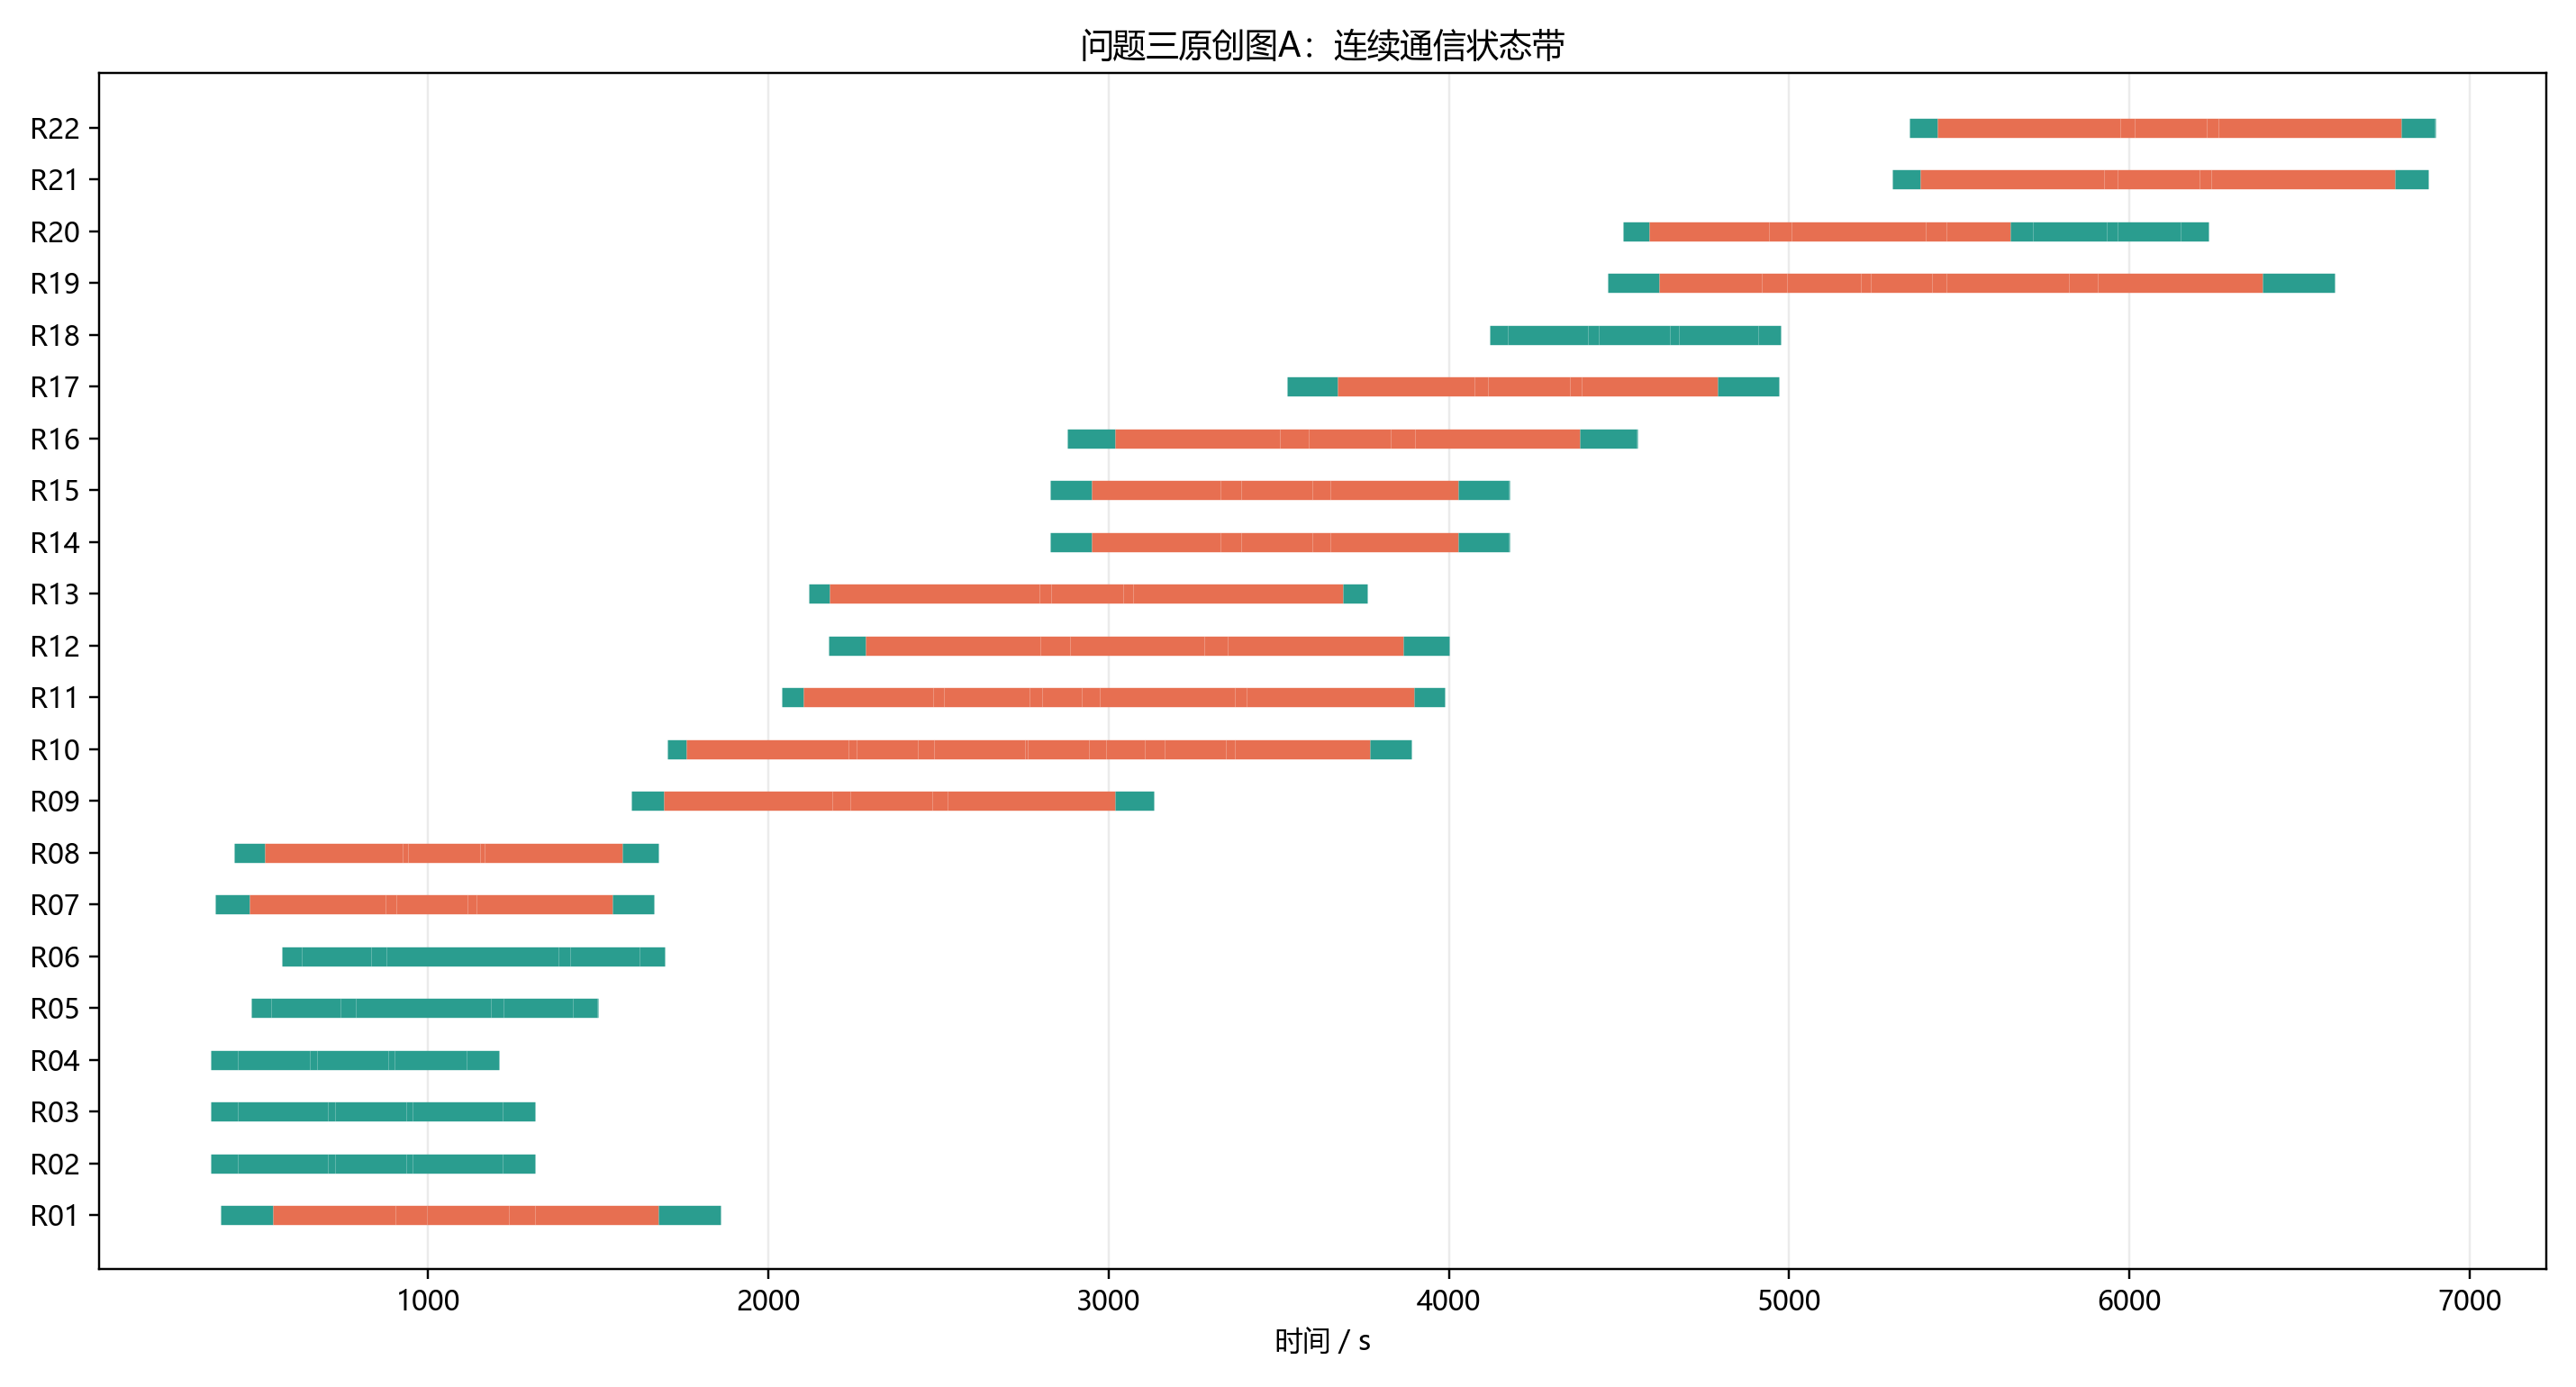
\includegraphics[width=0.98\textwidth]{问题三_原创图A_通信状态带.png}\caption{运输路线、中继悬停点和通信空间关系}\end{figure}
\begin{figure}[H]\centering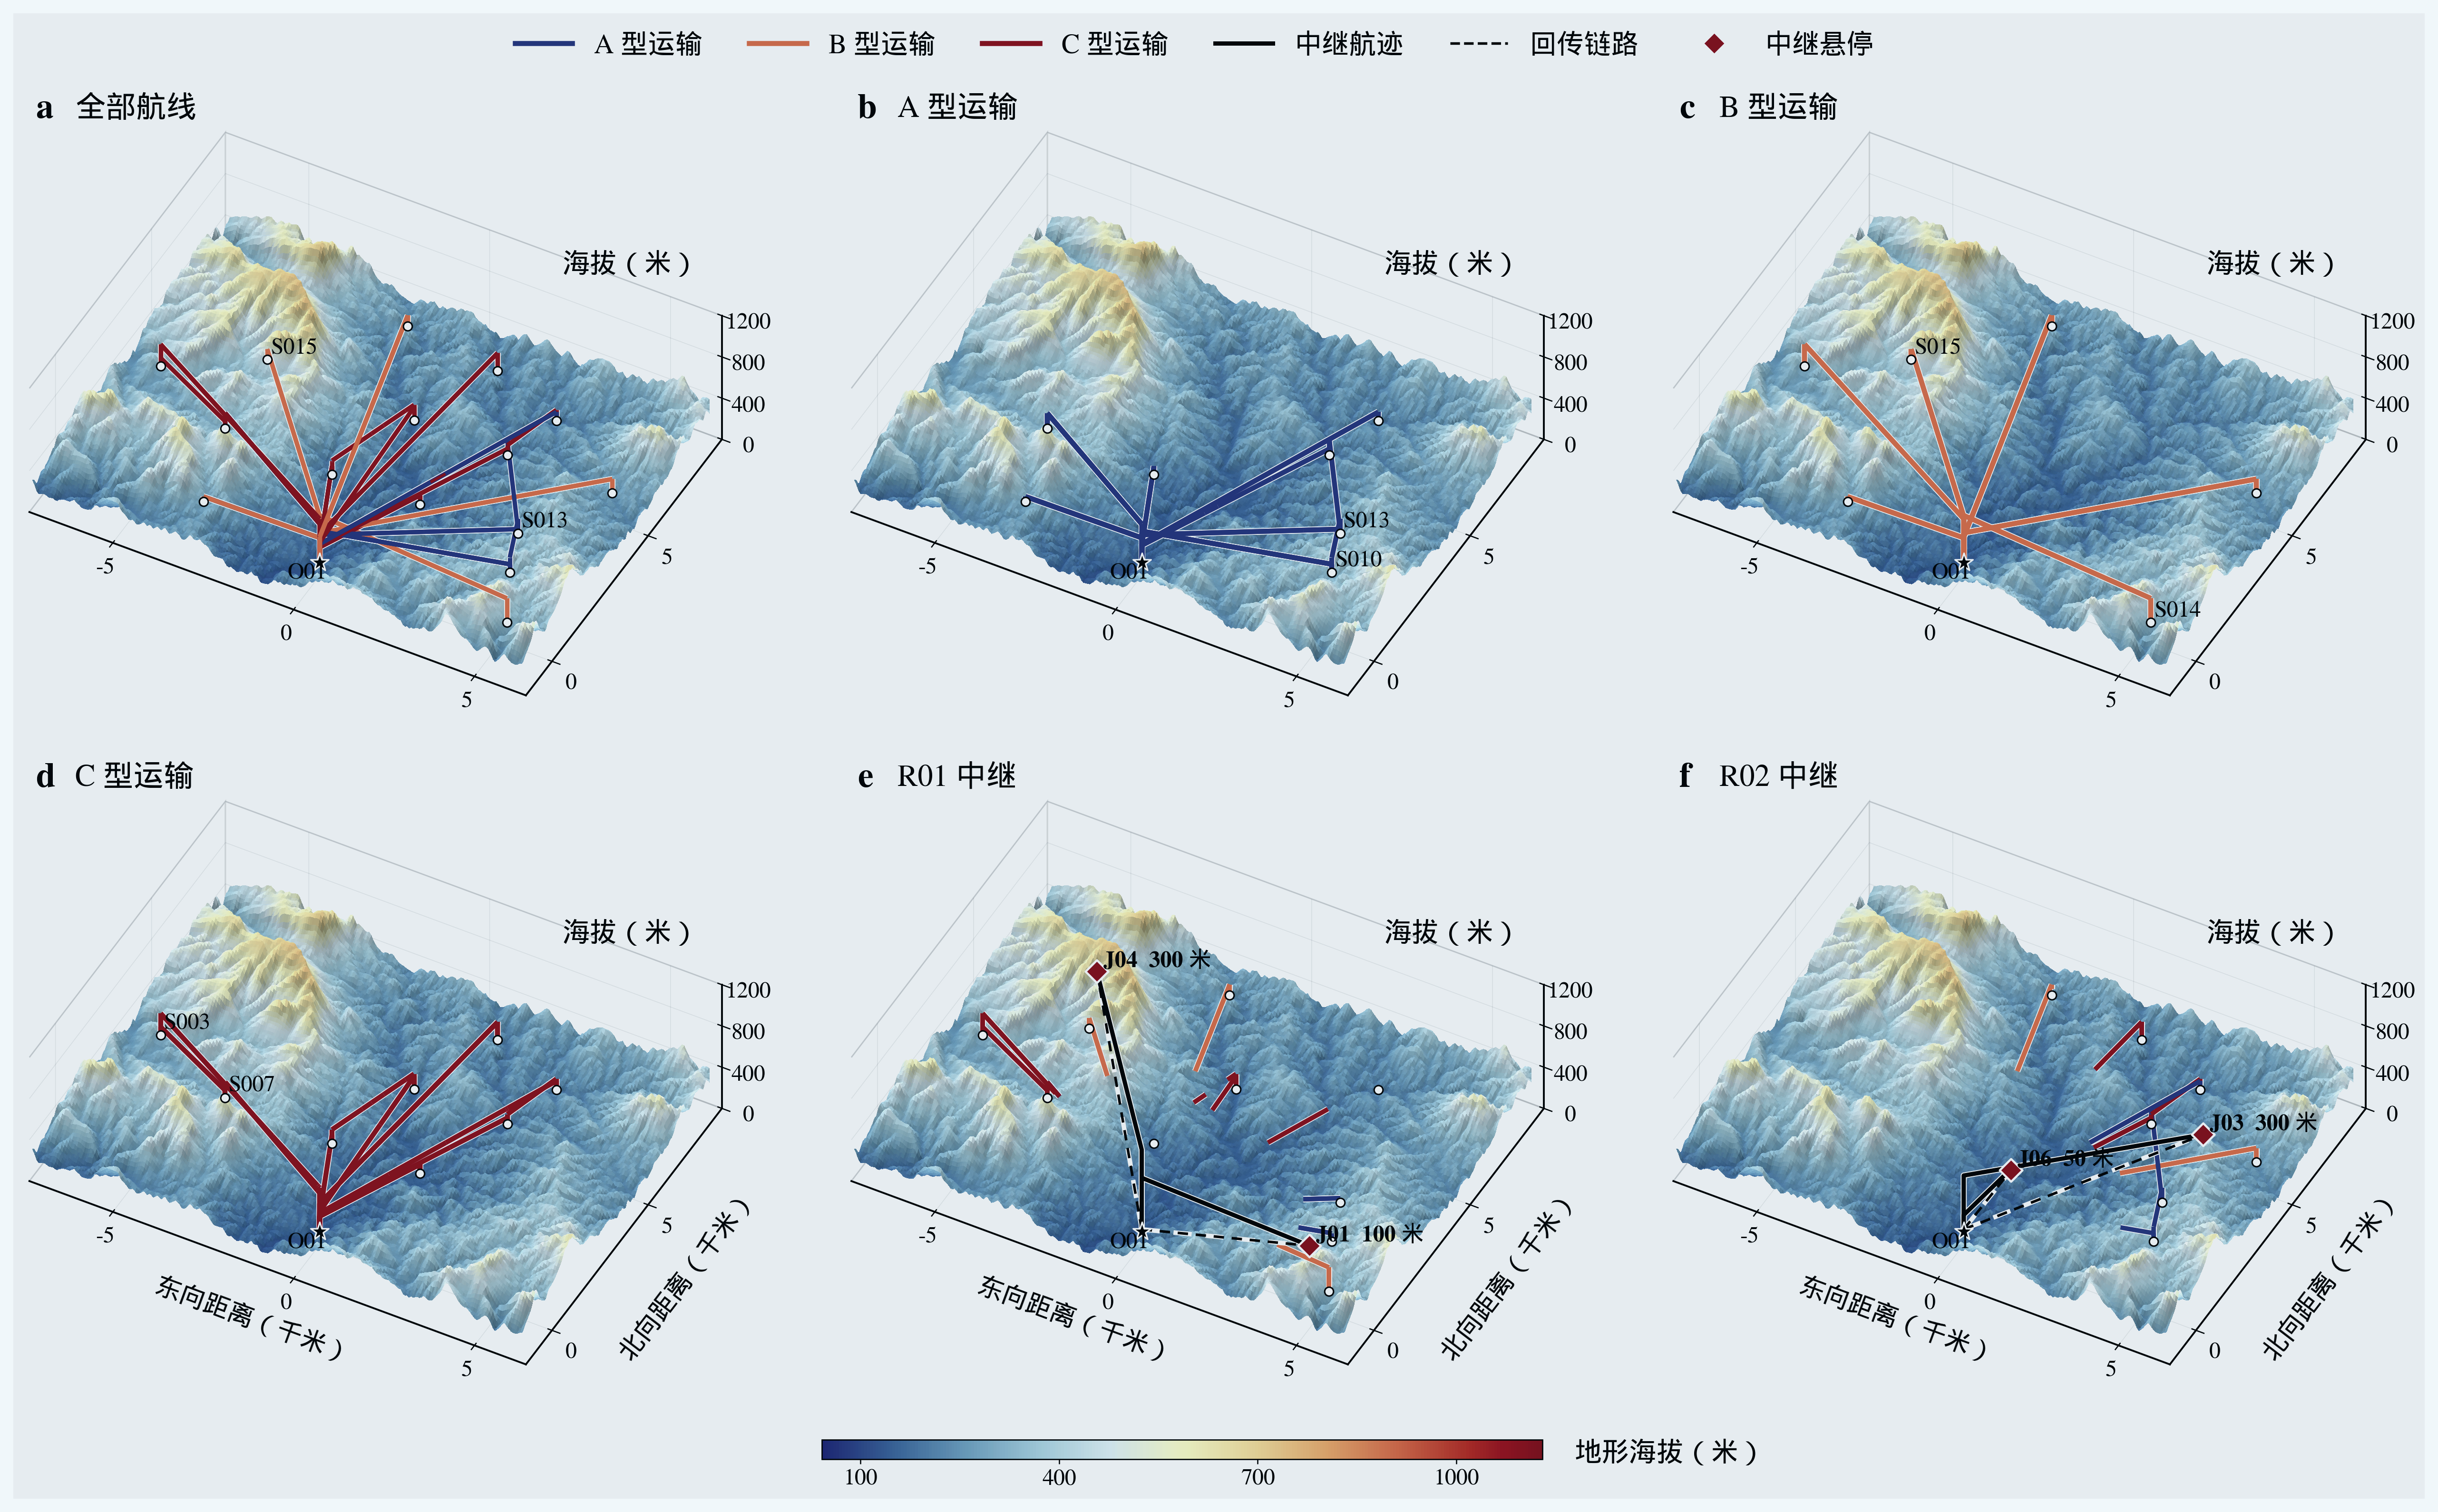
\includegraphics[width=0.98\textwidth]{问题三_时间主方案_三维_图03_六面板三维山地航线.png}\caption{三维山地轨迹与分层航线}\end{figure}
\begin{figure}[H]\centering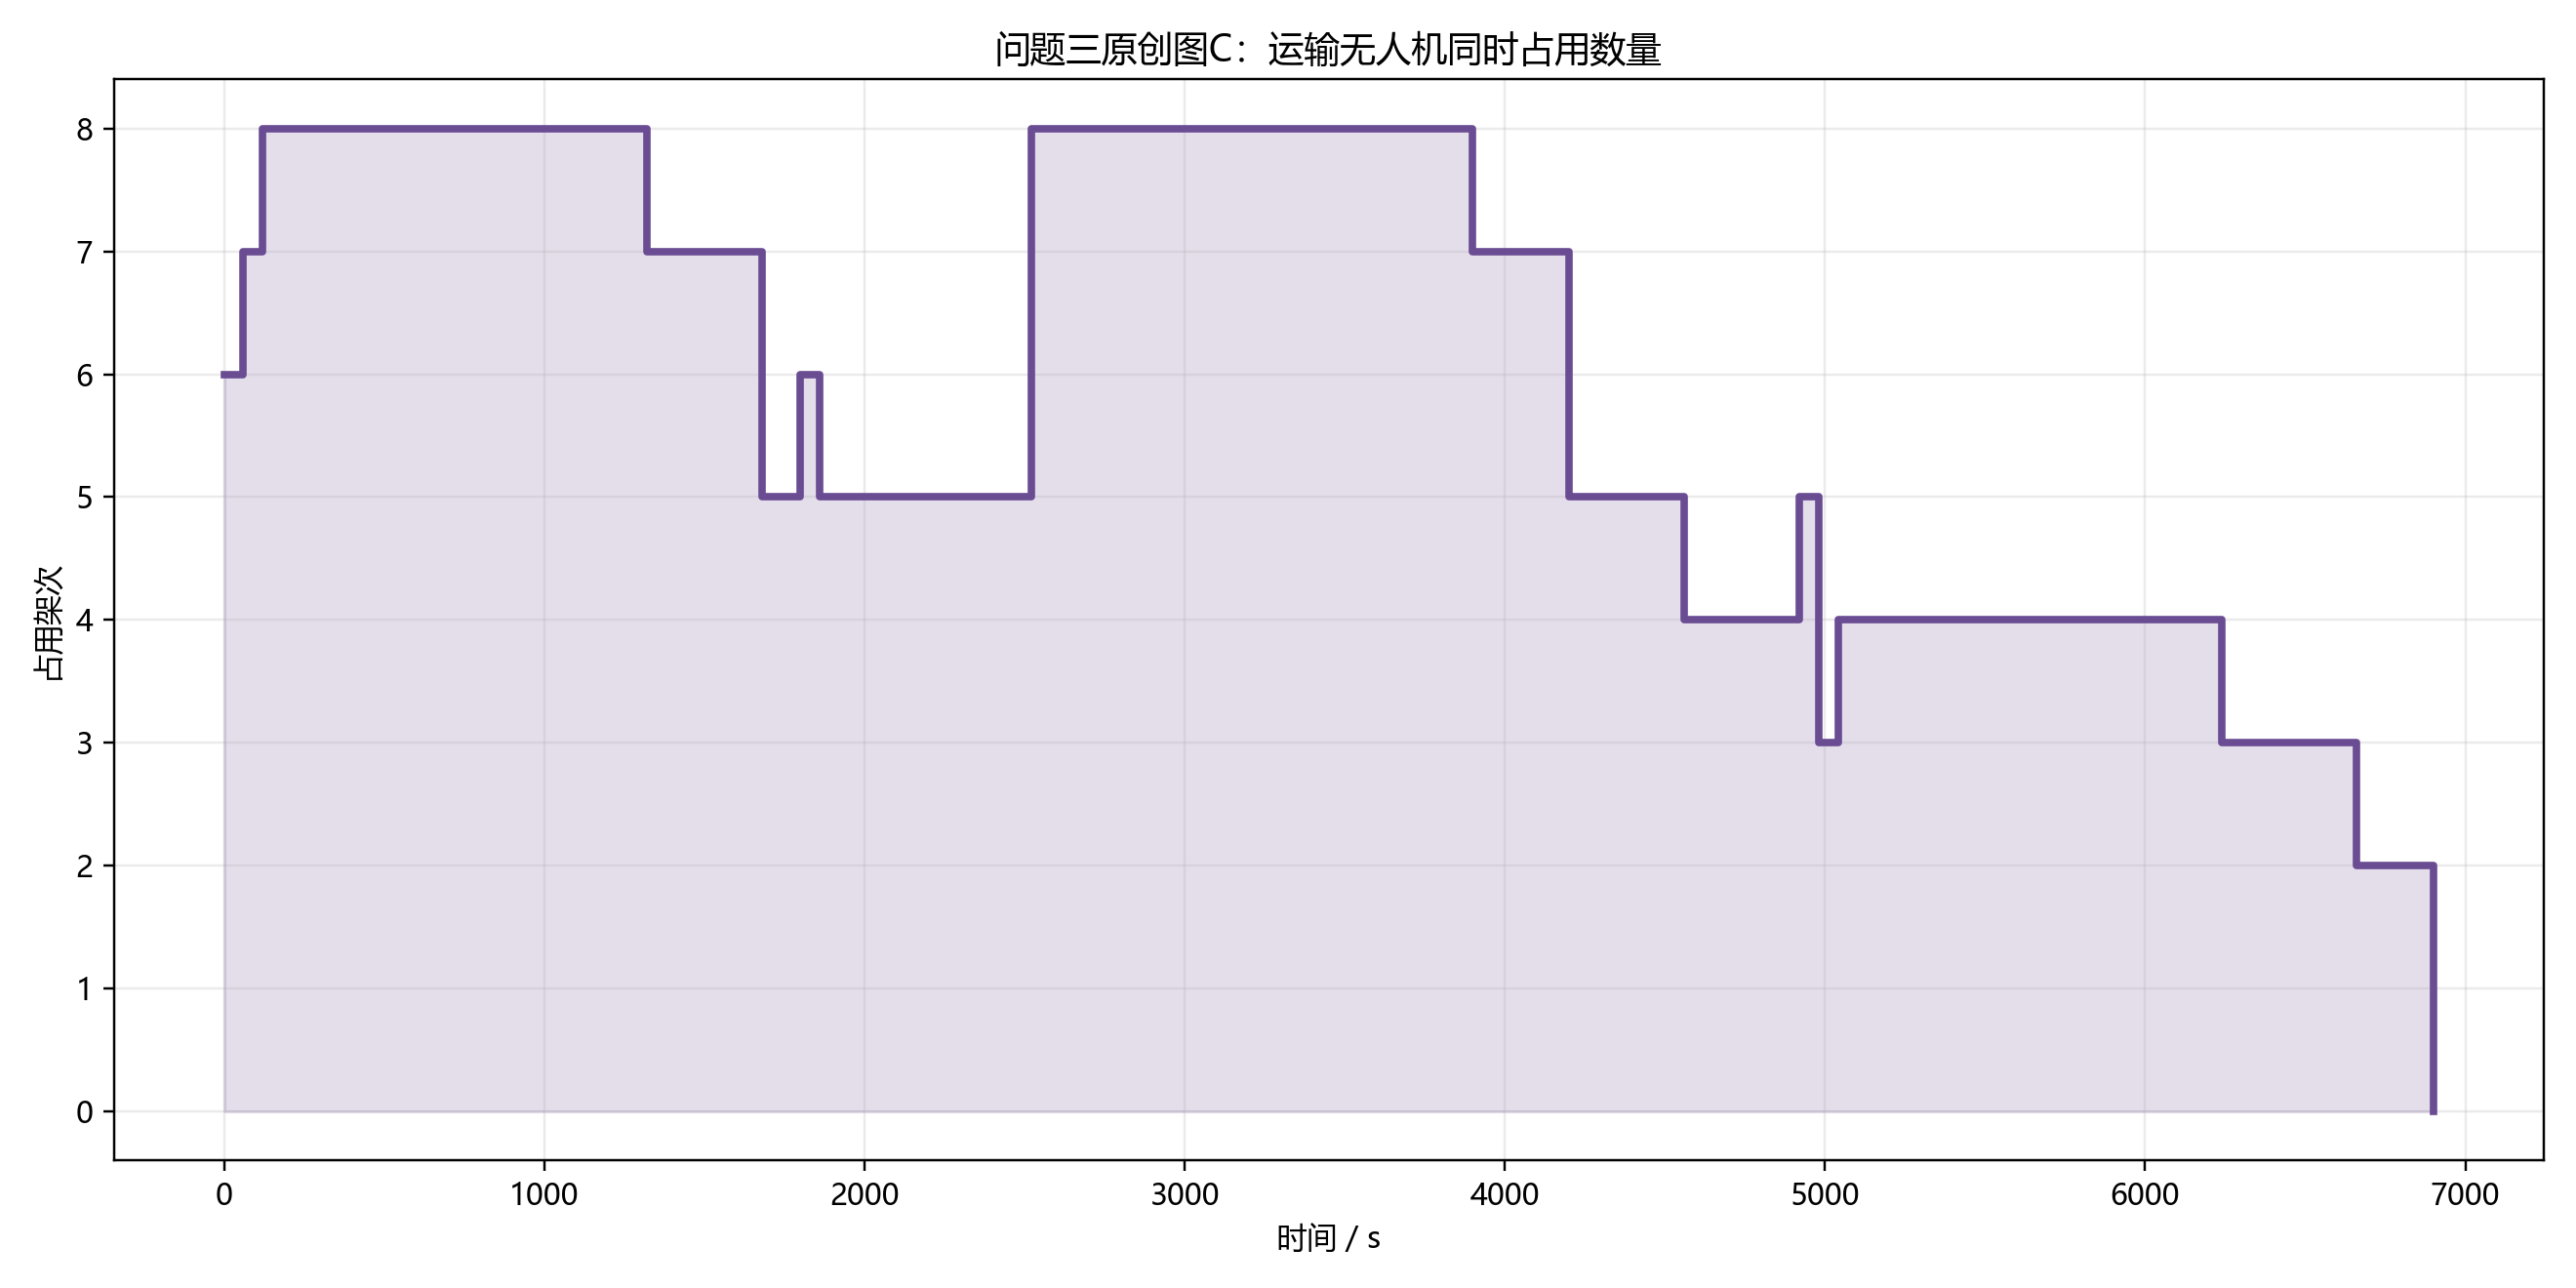
\includegraphics[width=0.98\textwidth]{问题三_原创图C_资源负载.png}\caption{运输与中继联合资源时序}\end{figure}
\begin{figure}[H]\centering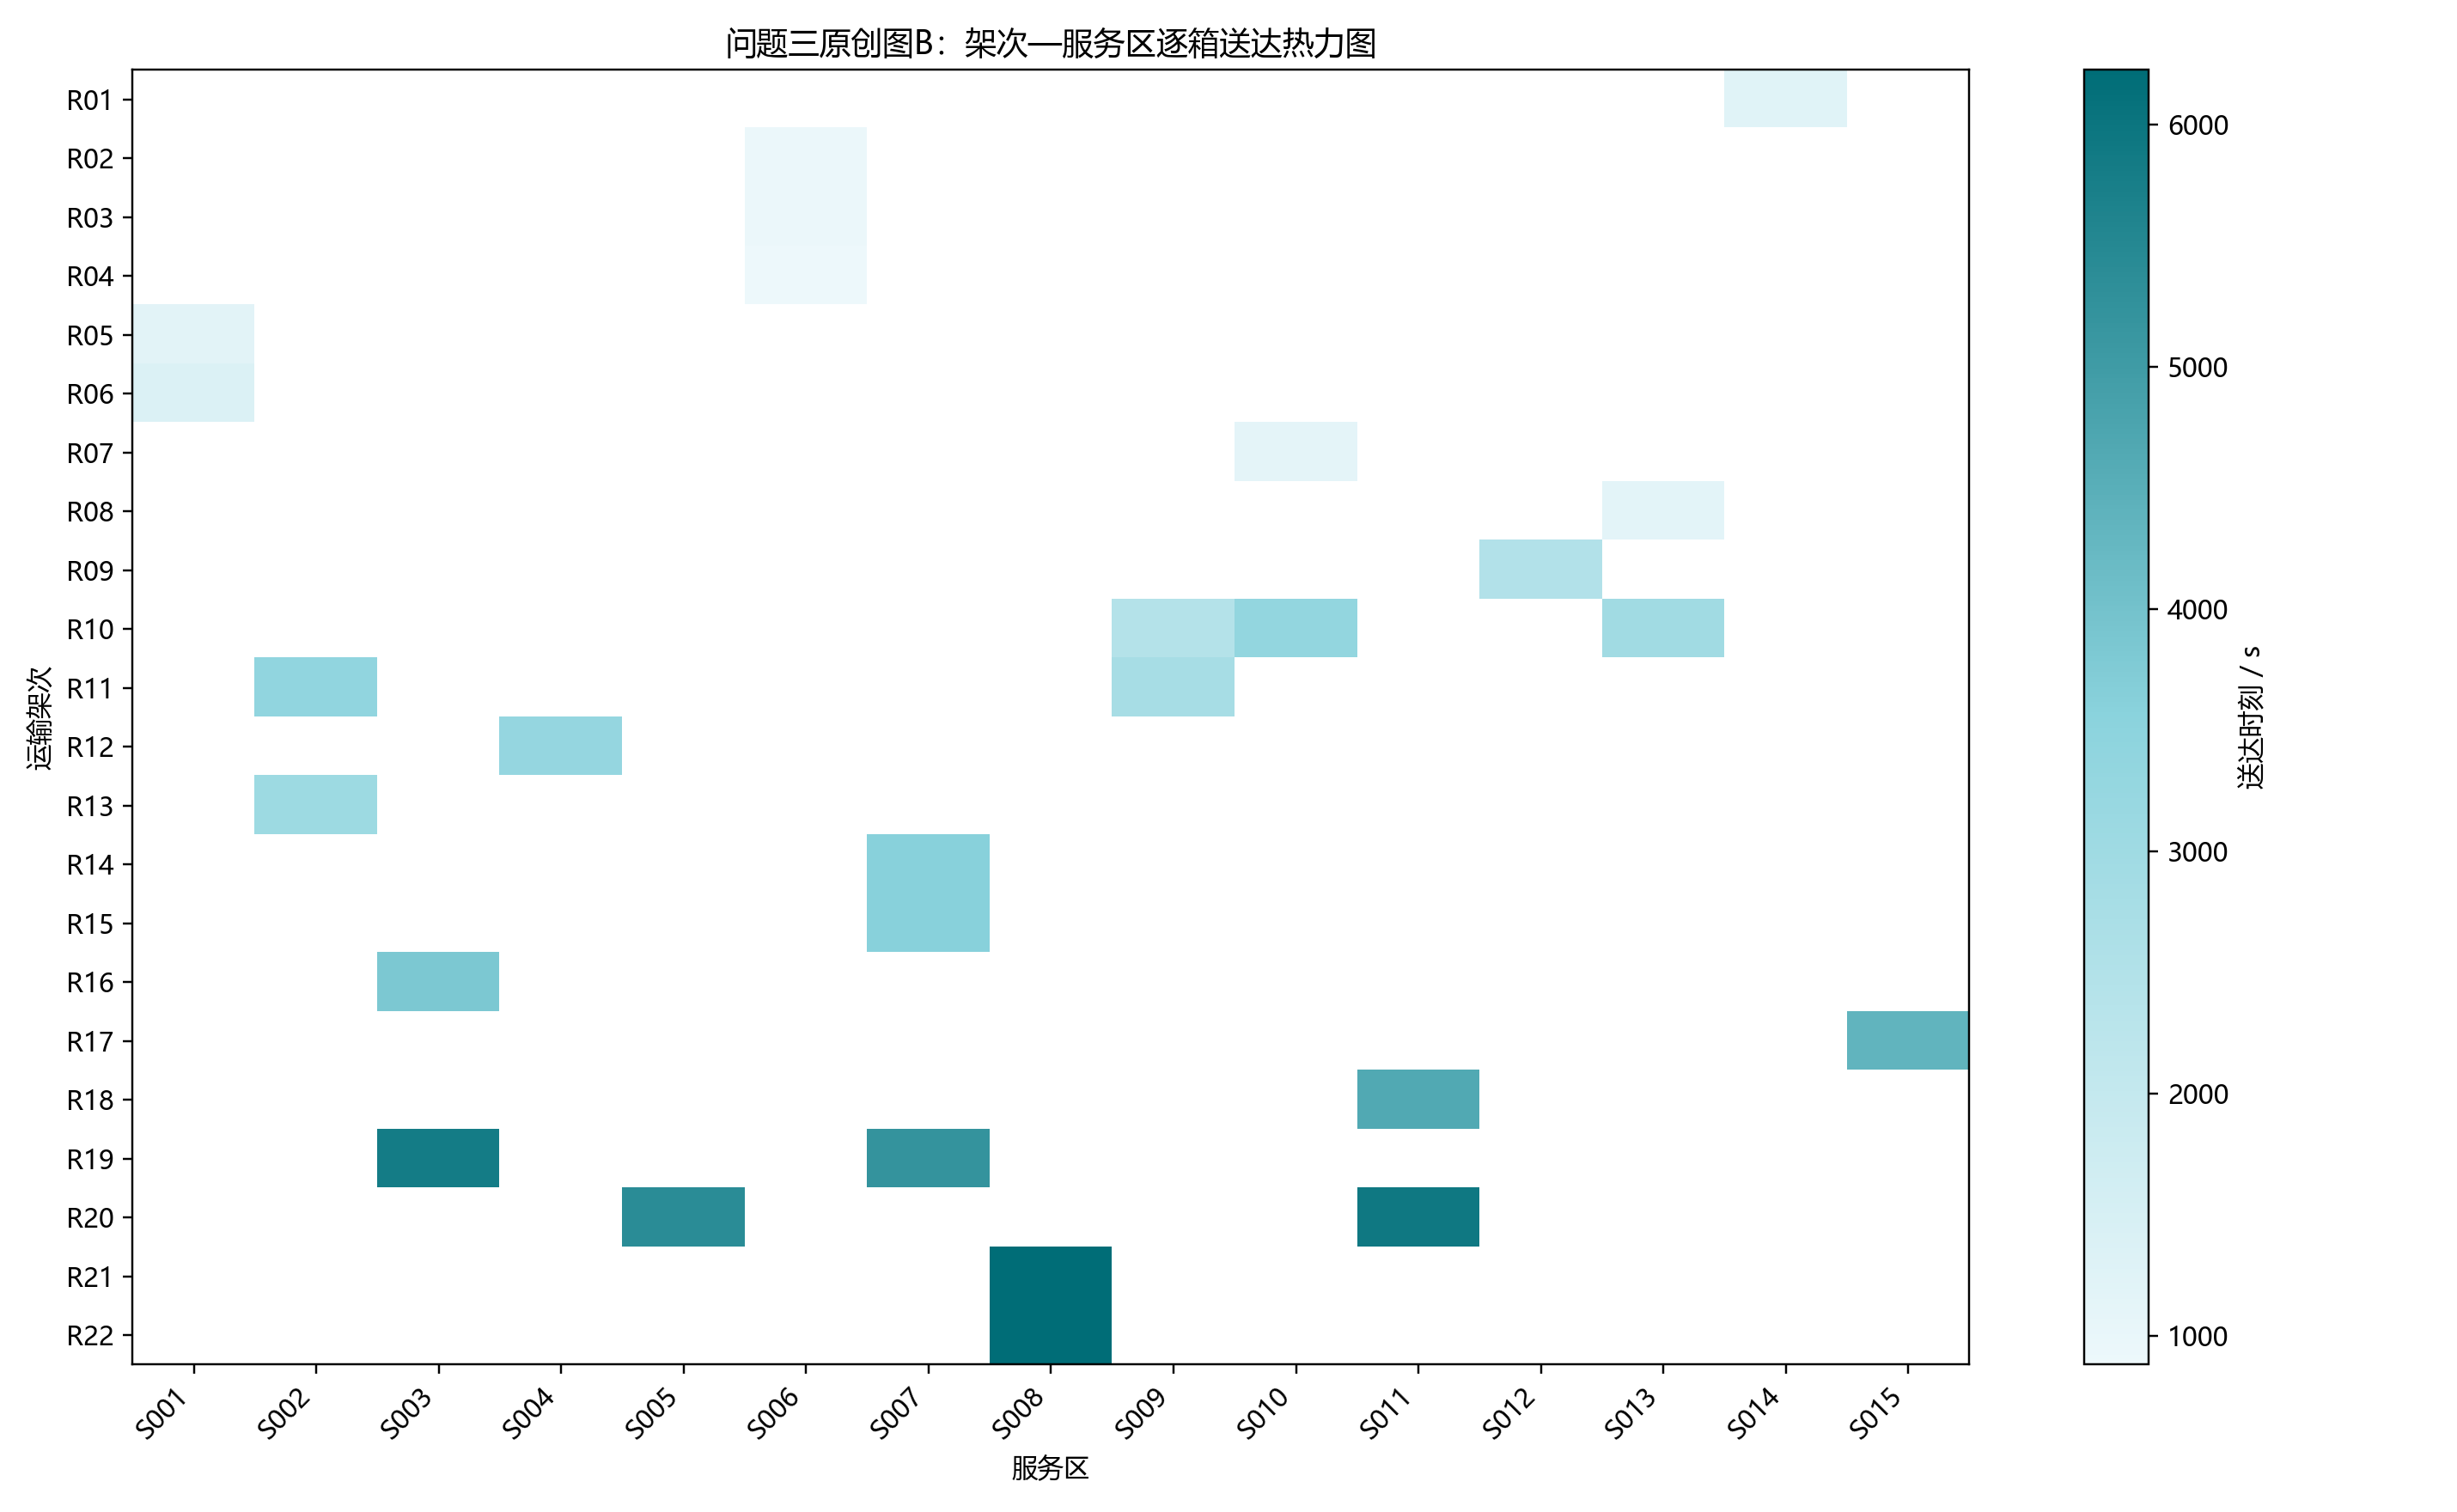
\includegraphics[width=0.98\textwidth]{问题三_原创图B_送达热力图.png}\caption{逐箱交付和资源核验}\end{figure}

架次安排、逐箱送达和通信关系不在正文中重复抄写，统一引用以下机器可读文件：\texttt{问题三结果/问题三\_时间主方案\_运输\_架次.csv}、\texttt{问题三\_时间主方案\_运输\_逐箱.csv}、\texttt{问题三\_时间主方案\_精确\_通信提交记录.csv}、\texttt{问题三\_时间主方案\_精确\_连续通信复核.json}。这些文件与正文指标采用同一 SHA256 数据链。

\section{参数扰动与稳健性分析}

\subsection{返航安全余量}
返航余量比例由 $\rho_g$ 增大时，运输架次的允许能耗上限 $(1-\rho_g)E_g^{\mathrm{use}}$ 下降，重载多点架次可能被拆分，运输架次和电池周转时间增加。建议对 $\rho_g\in\{0.15,0.20,0.25,0.30\}$ 重算问题二候选和问题三通信覆盖；输出架次、$C_{\max}$、能耗、最小 SOC 和中继架次。当前主方案使用题目给定的 $\rho_g=0.20$，不能用改变余量后的结果替代主方案。

\subsection{通信参数}
增大接收灵敏度门限、衰落裕量或遮挡附加损耗会缩小直连和中继链路的可行区域。对每个参数扰动，重新生成通信原子区间和候选覆盖集合，再求解集合覆盖；不能只在原通信标签上乘一个比例。可记录中继点数、服务总时长、通信中断秒数、联合完成时间和总能耗。

\subsection{悬停高度与中继资源}
提高悬停离地上限通常扩大接入链路可行区，但会增加爬升、返航和能耗；降低上限则可能增加中继架次。将 $h_{\max}$、中继无人机数量和能源组件数量分别做单因素扫描，若资源峰值超过库存，则报告最小缺口而不强行删去通信任务。

\subsection{充电时间与多目标权重}
充电时间增加会首先影响共享电池和中继能源组件周转，可能使 $C_{\max}$ 增加而不改变飞行时间。权重分析不应声称存在唯一最优方案：可用 $\varepsilon$-约束固定零延误，分别扫描 $C_{\max}$ 上界和能耗上界，形成运输及时性--完成时间--能耗--架次的 Pareto 候选集合。

\section{资源可行性检查清单}

\begin{enumerate}
\item 80 个货箱逐箱唯一覆盖，质量和体积约束全部通过；
\item 医疗和首批保障硬时限全部满足，普通货箱零延误；
\item 运输无人机峰值 $4/2/2$ 不超过库存；
\item 运输共享电池峰值 $6/4/4$ 不超过库存，复用前均已充满；
\item 中继无人机峰值 $2$ 不超过 R01/R02 两架库存；
\item 中继能源组件峰值 $3$ 不超过 6 组库存；
\item 所有运输和中继返航安全余量满足；
\item 223 个物理阶段、468 个解析区间通信状态连续，无中断；
\item 联合完成时间为所有运输和中继返航时刻的最大值，即 $6936\,\mathrm{s}$。
\end{enumerate}

\section{结论}

问题三不能把问题二的运输排班直接当作最终答案，而应在其货箱组批和运输候选基础上加入连续通信约束，重新确定中继悬停点、服务窗口和资源轮换。本文采用“通信预计算--集合覆盖初解--CP-SAT 时序优化--解析连续通信复核”的方法，得到 22+4 主方案。该方案 80 箱全部按期、通信中断为 0、联合完成时间 6936 s、总能耗 66.215521 kWh，并通过运输、中继、电池、能源组件和 DEM 独立核验。其最优性范围限定为当前候选路线、候选悬停点和固定物理规则下的已验证方案，不宣称完整连续空间 MINLP 的全局最优。

\maketitle\tableofcontents
\section{题意与继承边界}
问题四在问题三方案基础上改变任务组织方式。本文严格继承问题三已经核验的货箱组批、服务区访问顺序、运输架次、逐箱送达时刻、通信保障关系及中继服务窗口；问题四不重新安排飞行时刻，也不把问题三中的一架无人机在同一时段同时分配给多个独立组。这样处理保证第四问的比较对象是同一个已验证任务，而不是重新求解了一个不同的问题。

题目原始条件只要求每个独立组至少包含一个服务区。因此，论文同时给出“严格冻结口径”和“增配后独立执行口径”。前者用于回答现有库存是否足以完成分组；后者用于说明若允许复制跨组中继模板，最少需要增加哪些设备。两种口径的资源数字不混合。

\section{联合任务块的构造}
令 $V$ 为 15 个服务区，$P$ 为问题三运输架次集合，$R$ 为中继服务架次集合。若同一运输架次访问服务区 $i,j$，则加入超边 $e_p=\{i,j,\ldots\}$；若同一中继服务窗口同时保障多个服务区对应的运输段，则加入通信超边 $e_r$。由全部超边构成超图 $H=(V,E)$。对 $H$ 做并查集合并，得到不可拆任务块
\[
B_1=\{S001\},\quad B_2=\{S006\},\quad B_3=\{S002,S003,S004,S005,S007,S008,S009,S010,S011,S012,S013,S014,S015\}.
\]
不可拆的含义是：若将同一超边拆到不同组，至少有一架运输机或一条通信链路必须跨组调度，从而违反独立执行假设。因此后续分区只在 $\{B_1,B_2,B_3\}$ 的块级集合上进行。

\section{资源需求模型}
对组 $k$ 和资源类型 $h$，令 $n_{kh}$ 为专属资源需求，$N_h$ 为库存。运输机和电池占用区间分别为 $[s_p,e_p]$ 与 $[s_p,c_p]$；中继机和能源组件占用区间分别为 $[a_r,d_r]$ 与 $[a_r,f_r]$。对同组任意时刻 $t$，若区间集合中同时包含 $q$ 个任务，则必须有
\[
q\le n_{kh}.
\]
因此 $n_{kh}$ 至少等于对应区间图的最大团数。采用按开始时刻排序的贪心着色，所得颜色数等于区间图最大重叠数，故在固定时序下该配置是最小专属配置，而不是求解器随意给出的上界。库存缺口定义为
\[
\Delta_h=\max\{0,\sum_k n_{kh}-N_h\}.
\]

\section{严格冻结口径结果}
原题允许的分区枚举结果如下。
\begin{table}[H]\centering\caption{严格冻结口径下的分区比较}
\begin{tabular}{llll}\toprule
方案&分区结构&库存缺口&结论\\\midrule
K2-01&$S006$ / 其余14区&6&缺口较小，但含单站组\\
K2-02&$S001,S006$ / 其余13区&10&无单站组，负载较均衡\\
K2-03&$S001$ / 其余14区&4&原始条件下缺口最小，但含单站组\\
K3-01&$S001$ / 13区 / $S006$&10&若要求每组至少2区则不可用\\\bottomrule
\end{tabular}\end{table}

这里必须区分两个结论：若优化目标只有库存缺口，K2-03 的缺口 4 件最小；若组织规则附加要求每组至少两个服务区，K2-02 是唯一块级结构。不能将后一个附加偏好写成题目原始硬约束。

\section{增配后的独立执行方案}
为使不同组真正能够同时独立执行，若某个中继模板服务了多个组，则对每个组复制该模板的悬停点、服务时段和能源组件占用，并将复制任务重新计入资源峰值与能耗。以库存缺口优先、再以运输工时公平性为次级目标，得到推荐二组方案：
\begin{itemize}
\item $G_1=\{S001,S002,S004,S005,S009,S010,S011,S013\}$，47 箱，10 个运输架次；
\item $G_2=\{S003,S006,S007,S008,S012,S014,S015\}$，33 箱，12 个运输架次。
\end{itemize}
两组运输工时为 19271 s 与 21430 s，归一化 Gini 系数为 0.0530；复制中继模板后中继架次为 7，联合完成时间仍为 6936 s，最后送达仍为 6227 s，总能耗为 68.710272 kWh。资源需求和缺口为：A 型运输机 $5/4$、B 型 $2/2$、C 型 $3/2$；A/B/C 型电池 $6/6$、$4/4$、$5/4$；中继机 $4/2$，中继能源组件 $6/6$。故最小增配为 1 架 A 型运输机、1 架 C 型运输机、1 组 C 型电池和 2 架中继无人机，共 5 件。

作为三组备选，分区为 $(S001,S003,S006,S007)$、$(S002,S005,S009,S010,S011,S013)$ 和 $(S004,S008,S012,S014,S015)$，运输工时 Gini 为 0.0819，复制后中继架次为 8，总能耗 69.968349 kWh，库存缺口为 9 件。因此三组方案的组织粒度更细，但资源代价和能耗均劣于二组方案。

\section{优化目标与算法}
分区的字典序目标为：第一，满足每组独立执行的硬约束；第二，最小化总库存缺口 $\sum_h\Delta_h$；第三，最小化组间运输工时的归一化 Gini 系数；第四，最小化复制中继带来的附加能耗。块级枚举保证了结构完整性，区间图着色给出每组资源的最小需求，最后用 CP-SAT 对区间不重叠和资源上界进行独立核验。该流程比直接按地理距离聚类更严格，因为通信超边会禁止表面上相近但通信上不可拆的服务区被分开。

\section{敏感性与可行性检验}
在严格冻结口径下，改变组数只改变块的组合方式，不会改变问题三的逐箱时刻和通信判定。对推荐增强方案，分别增加或减少一架中继机、一个能源组件和一组 C 型电池，重新计算区间峰值即可得到资源缺口的边际变化。由于推荐方案的运输工时 Gini 仅为 0.0530，三组方案反而出现 9 件缺口，说明在本数据下继续细分任务并不能提高独立执行能力。

最终核验清单为：所有服务区恰分配一次；任何运输架次不跨组；通信中继模板不跨组复用；区间资源无重叠；医疗、首批和其他货箱仍使用问题三的按期送达记录；联合完成时间和中继服务窗口与问题三一致；库存缺口逐项列明且无负数资源被默许。

\section{结论}
严格冻结口径下，原始库存不能支持无增配的多组独立执行；K2-03 仅在允许单站组时具有最小库存缺口，K2-02 是禁止单站组时的唯一块级结构。若允许复制跨组中继模板，推荐二组 8/7 服务区方案，缺口 5 件、工时 Gini 0.0530、总能耗 68.710272 kWh。该结论同时报告了题目原始条件下的严格可行性和增配后的工程执行方案，避免把附加组织偏好误写成题目约束。

\section{问题四可视化结果}
问题四的图件直接对应分区枚举、地形空间关系和资源峰值计算。图~\ref{fig:q4map} 展示两组、三组分区及服务区位置；图~\ref{fig:q4terrain} 展示固定航线与三维地形关系；图~\ref{fig:q4gap} 展示不同方案的资源缺口；图~\ref{fig:q4time} 展示资源峰值时间分布。
\begin{figure}[H]\centering\includegraphics[width=0.92\textwidth]{问题四_图01_原色带DEM_两组三组分区.png}\caption{问题四分区方案与 DEM 空间分布}\label{fig:q4map}\end{figure}
\begin{figure}[H]\centering\includegraphics[width=0.92\textwidth]{问题四_图02_原视角三维地形与固定航线.png}\caption{固定航线与三维山地地形}\label{fig:q4terrain}\end{figure}
\begin{figure}[H]\centering\includegraphics[width=0.92\textwidth]{问题四_图03_原版三维地形与八类资源缺口.png}\caption{三维地形及资源缺口空间关联}\label{fig:q4gap}\end{figure}
\begin{figure}[H]\centering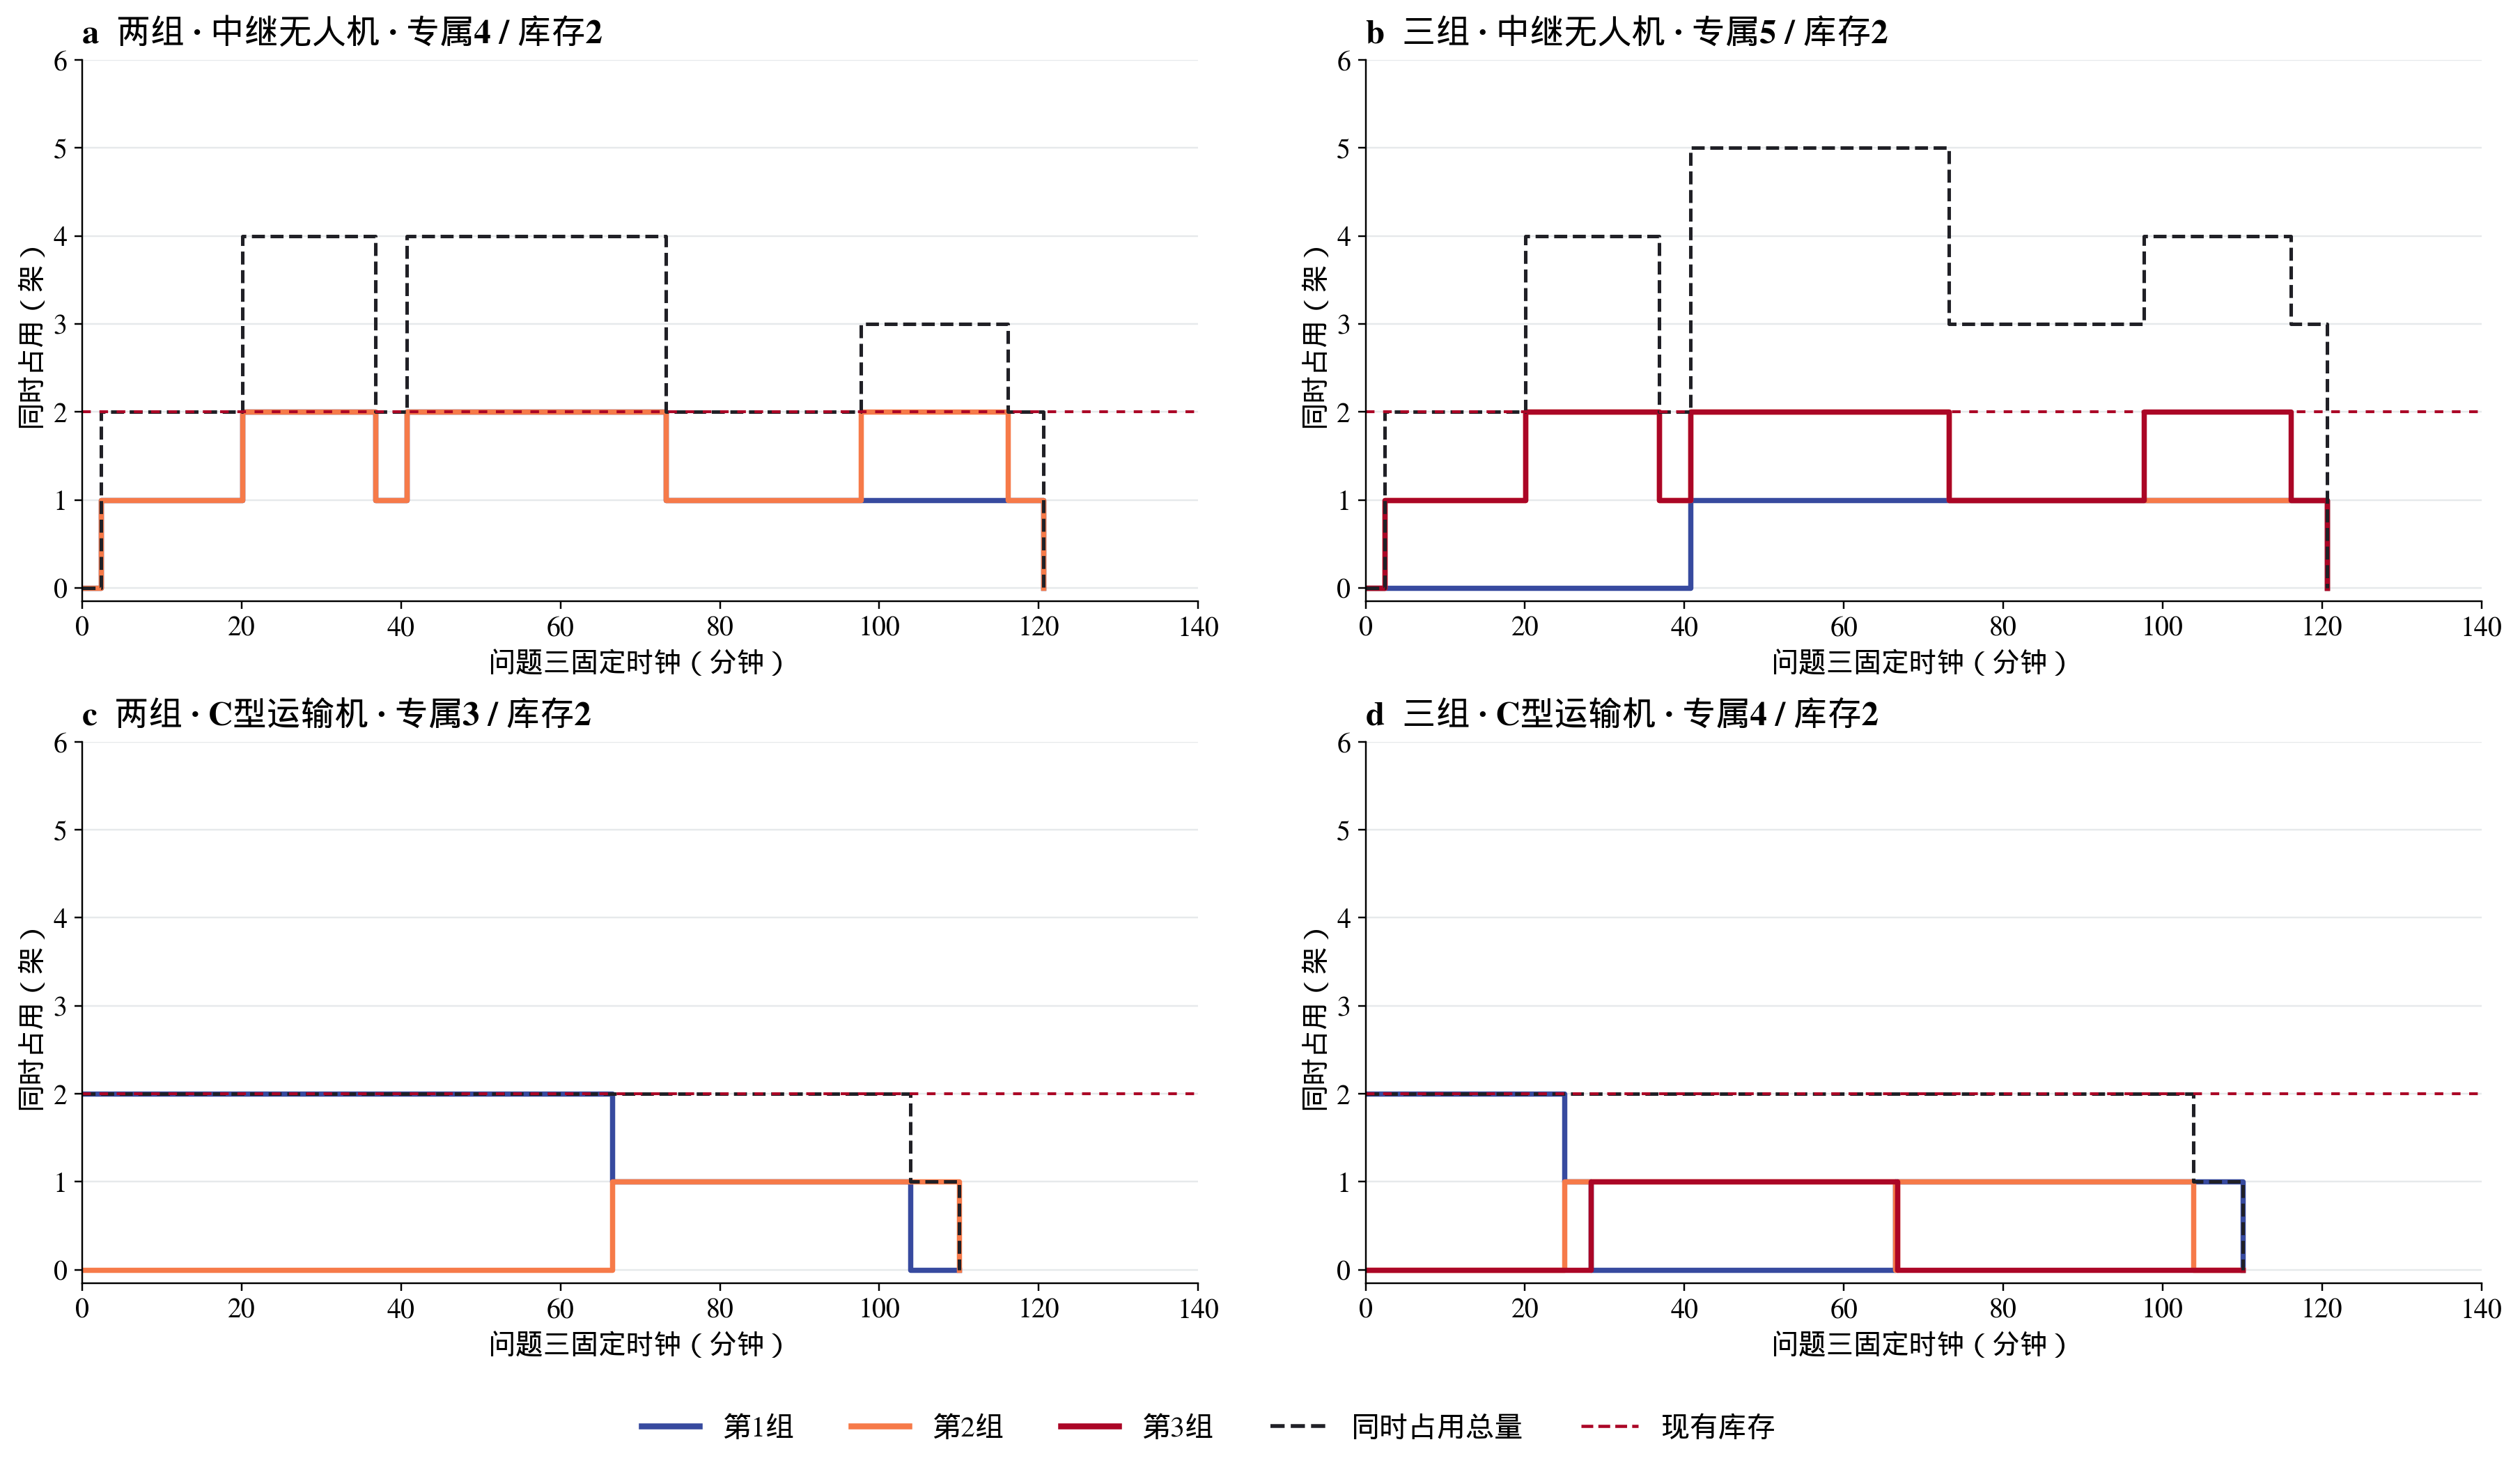
\includegraphics[width=0.92\textwidth]{问题四_图06_原版时序资源峰值.png}\caption{问题四资源占用峰值时间轴}\label{fig:q4time}\end{figure}`n\end{document}








